\documentclass{standalone}
\usepackage{tikz}
\usetikzlibrary{patterns, positioning}
\usepackage[sfdefault]{ClearSans} %% option 'sfdefault' activates Clear Sans as the default text font
\usepackage[T1]{fontenc}

\begin{document}
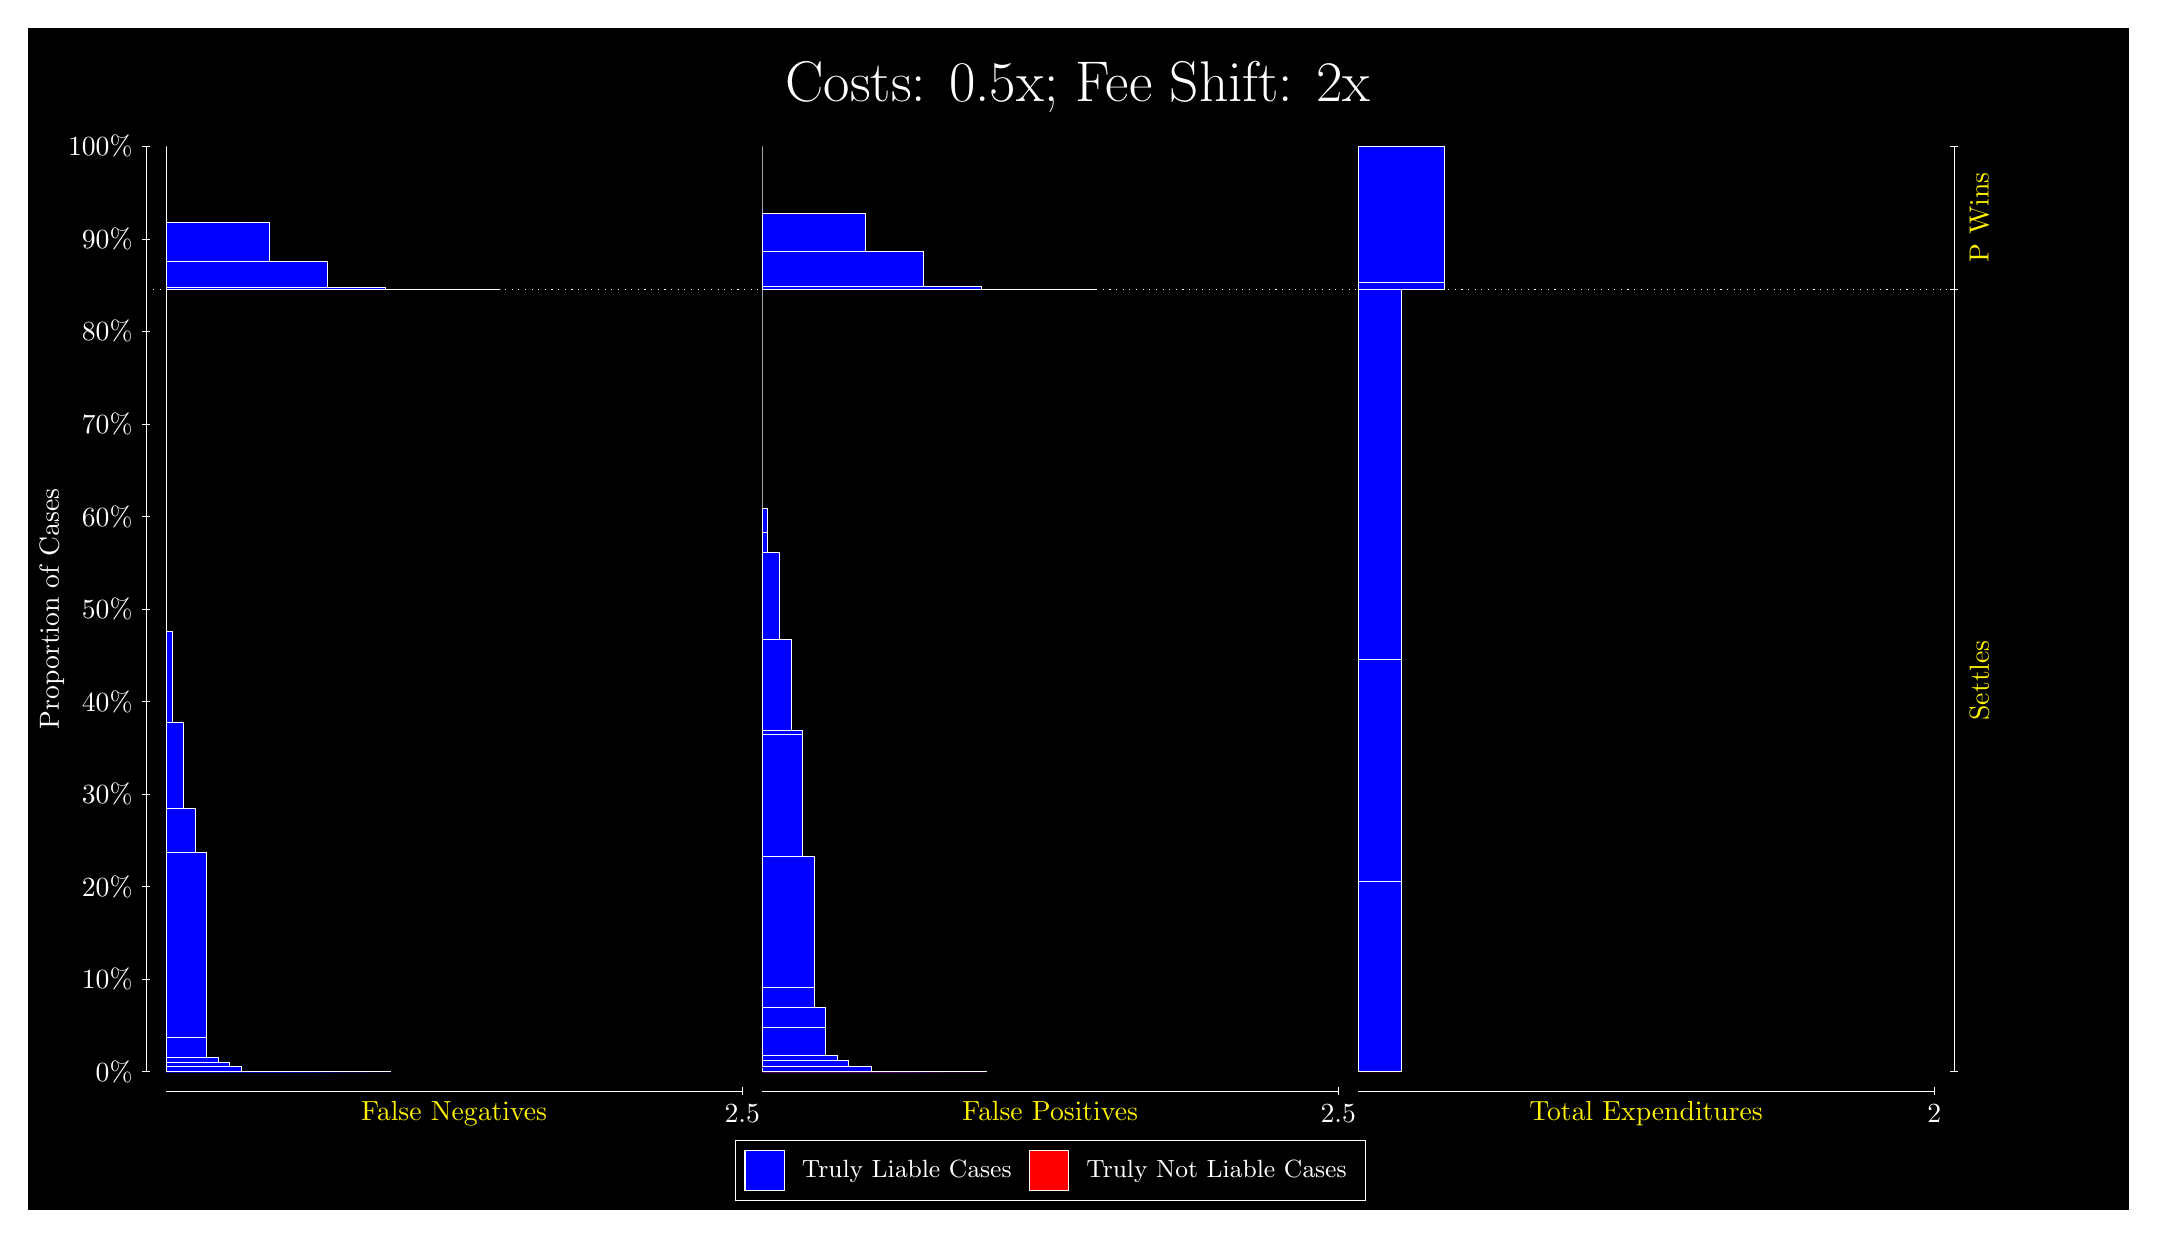
\begin{tikzpicture}
\draw[fill=black] (0,0) rectangle (26.667,15);
\draw[text=white] (0,13.5) rectangle (26.667,15) node[midway] {\huge Costs: 0.5x; Fee Shift: 2x};
\draw[white, very thin] (1.5,1.75) -- (1.5,13.5);
\node[rotate=90, text=white, anchor=center] at (0.3, 7.625) {Proportion of Cases};
\draw[white, very thin] (1.45,1.75) -- (1.55,1.75);
\node[text=white, anchor=east] at (1.45, 1.75) {0\%};
\draw[white, very thin] (1.45,2.925) -- (1.55,2.925);
\node[text=white, anchor=east] at (1.45, 2.925) {10\%};
\draw[white, very thin] (1.45,4.1) -- (1.55,4.1);
\node[text=white, anchor=east] at (1.45, 4.1) {20\%};
\draw[white, very thin] (1.45,5.275) -- (1.55,5.275);
\node[text=white, anchor=east] at (1.45, 5.275) {30\%};
\draw[white, very thin] (1.45,6.45) -- (1.55,6.45);
\node[text=white, anchor=east] at (1.45, 6.45) {40\%};
\draw[white, very thin] (1.45,7.625) -- (1.55,7.625);
\node[text=white, anchor=east] at (1.45, 7.625) {50\%};
\draw[white, very thin] (1.45,8.8) -- (1.55,8.8);
\node[text=white, anchor=east] at (1.45, 8.8) {60\%};
\draw[white, very thin] (1.45,9.975) -- (1.55,9.975);
\node[text=white, anchor=east] at (1.45, 9.975) {70\%};
\draw[white, very thin] (1.45,11.15) -- (1.55,11.15);
\node[text=white, anchor=east] at (1.45, 11.15) {80\%};
\draw[white, very thin] (1.45,12.325) -- (1.55,12.325);
\node[text=white, anchor=east] at (1.45, 12.325) {90\%};
\draw[white, very thin] (1.45,13.5) -- (1.55,13.5);
\node[text=white, anchor=east] at (1.45, 13.5) {100\%};

\draw[white, very thin] (24.457,1.75) -- (24.457,13.5);
\draw[white, very thin] (24.407,1.75) -- (24.507,1.75);
\node[anchor=west] at (24.407, 1.75) {};
\draw[white, very thin] (24.407,11.685) -- (24.507,11.685);
\node[anchor=west] at (24.407, 11.685) {};
\draw[white, very thin] (24.407,13.5) -- (24.507,13.5);
\node[anchor=west] at (24.407, 13.5) {};

\draw[white, very thin, fill=blue] (1.75,1.75) rectangle (4.6044,1.75);
\draw[white, very thin, fill=blue] (1.75,1.75) rectangle (4.3116,1.75);
\draw[white, very thin, fill=blue] (1.75,1.75) rectangle (4.0188,1.75);
\draw[white, very thin, fill=blue] (1.75,1.75) rectangle (3.8725,1.75);
\draw[white, very thin, fill=blue] (1.75,1.75) rectangle (3.7261,1.75);
\draw[white, very thin, fill=blue] (1.75,1.75) rectangle (3.5797,1.75);
\draw[white, very thin, fill=blue] (1.75,1.75) rectangle (3.4333,1.75);
\draw[white, very thin, fill=blue] (1.75,1.75) rectangle (3.287,1.75);
\draw[white, very thin, fill=blue] (1.75,1.75) rectangle (3.1406,1.75);
\draw[white, very thin, fill=blue] (1.75,1.75) rectangle (2.9942,1.7505);
\draw[white, very thin, fill=blue] (1.75,1.7505) rectangle (2.8478,1.7548);
\draw[white, very thin, fill=blue] (1.75,1.7548) rectangle (2.7015,1.8131);
\draw[white, very thin, fill=blue] (1.75,1.8131) rectangle (2.5551,1.8734);
\draw[white, very thin, fill=blue] (1.75,1.8734) rectangle (2.4087,1.9344);
\draw[white, very thin, fill=blue] (1.75,1.9344) rectangle (2.2623,2.1868);
\draw[white, very thin, fill=blue] (1.75,2.1868) rectangle (2.2623,4.5291);
\draw[white, very thin, fill=blue] (1.75,4.5291) rectangle (2.1159,5.0936);
\draw[white, very thin, fill=blue] (1.75,5.0936) rectangle (1.9696,6.1894);
\draw[white, very thin, fill=blue] (1.75,6.1894) rectangle (1.8232,7.3459);
\draw[white, very thin, fill=red] (1.75,7.3459) rectangle (1.75,7.3459);
\draw[white, very thin, fill=blue] (1.75,7.3459) rectangle (1.75,11.685);
\draw[white, very thin, fill=blue] (1.75,11.685) rectangle (5.9949,11.685);
\draw[white, very thin, fill=blue] (1.75,11.685) rectangle (5.2631,11.685);
\draw[white, very thin, fill=blue] (1.75,11.685) rectangle (4.5312,11.705);
\draw[white, very thin, fill=blue] (1.75,11.705) rectangle (3.7993,12.042);
\draw[white, very thin, fill=blue] (1.75,12.042) rectangle (3.5065,12.042);
\draw[white, very thin, fill=blue] (1.75,12.042) rectangle (3.0674,12.536);
\draw[white, very thin, fill=blue] (1.75,12.536) rectangle (2.7746,12.536);
\draw[white, very thin, fill=blue] (1.75,12.536) rectangle (2.3355,12.537);
\draw[white, very thin, fill=blue] (1.75,12.537) rectangle (2.0428,12.539);
\draw[white, very thin, fill=red] (1.75,12.539) rectangle (1.75,12.539);
\draw[white, very thin, fill=blue] (1.75,12.539) rectangle (1.75,13.5);
\draw[white, very thin, fill=red] (9.3189,1.75) rectangle (12.173,1.75);
\draw[white, very thin, fill=blue] (9.3189,1.75) rectangle (12.173,1.75);
\draw[white, very thin, fill=red] (9.3189,1.75) rectangle (11.588,1.75);
\draw[white, very thin, fill=blue] (9.3189,1.75) rectangle (11.588,1.75);
\draw[white, very thin, fill=blue] (9.3189,1.75) rectangle (11.441,1.75);
\draw[white, very thin, fill=red] (9.3189,1.75) rectangle (11.295,1.75);
\draw[white, very thin, fill=blue] (9.3189,1.75) rectangle (11.295,1.75);
\draw[white, very thin, fill=red] (9.3189,1.75) rectangle (11.002,1.75);
\draw[white, very thin, fill=blue] (9.3189,1.75) rectangle (11.002,1.75);
\draw[white, very thin, fill=blue] (9.3189,1.75) rectangle (10.856,1.7505);
\draw[white, very thin, fill=red] (9.3189,1.7505) rectangle (10.709,1.7505);
\draw[white, very thin, fill=blue] (9.3189,1.7505) rectangle (10.709,1.7512);
\draw[white, very thin, fill=blue] (9.3189,1.7512) rectangle (10.709,1.8104);
\draw[white, very thin, fill=blue] (9.3189,1.8104) rectangle (10.563,1.8125);
\draw[white, very thin, fill=red] (9.3189,1.8125) rectangle (10.417,1.8125);
\draw[white, very thin, fill=blue] (9.3189,1.8125) rectangle (10.417,1.8978);
\draw[white, very thin, fill=blue] (9.3189,1.8978) rectangle (10.27,1.9566);
\draw[white, very thin, fill=red] (9.3189,1.9566) rectangle (10.124,1.9566);
\draw[white, very thin, fill=blue] (9.3189,1.9566) rectangle (10.124,2.3131);
\draw[white, very thin, fill=blue] (9.3189,2.3131) rectangle (10.124,2.5676);
\draw[white, very thin, fill=blue] (9.3189,2.5676) rectangle (9.9776,2.8207);
\draw[white, very thin, fill=blue] (9.3189,2.8207) rectangle (9.9776,4.4833);
\draw[white, very thin, fill=red] (9.3189,4.4833) rectangle (9.8312,4.4833);
\draw[white, very thin, fill=blue] (9.3189,4.4833) rectangle (9.8312,6.0306);
\draw[white, very thin, fill=blue] (9.3189,6.0306) rectangle (9.8312,6.0892);
\draw[white, very thin, fill=blue] (9.3189,6.0892) rectangle (9.6848,7.2458);
\draw[white, very thin, fill=blue] (9.3189,7.2458) rectangle (9.5384,8.3415);
\draw[white, very thin, fill=blue] (9.3189,8.3415) rectangle (9.3921,8.5946);
\draw[white, very thin, fill=blue] (9.3189,8.5946) rectangle (9.3921,8.906);
\draw[white, very thin, fill=blue] (9.3189,8.906) rectangle (9.3189,11.685);
\draw[white, very thin, fill=red] (9.3189,11.685) rectangle (13.564,11.685);
\draw[white, very thin, fill=blue] (9.3189,11.685) rectangle (13.564,11.685);
\draw[white, very thin, fill=red] (9.3189,11.685) rectangle (12.832,11.685);
\draw[white, very thin, fill=blue] (9.3189,11.685) rectangle (12.832,11.686);
\draw[white, very thin, fill=red] (9.3189,11.686) rectangle (12.1,11.686);
\draw[white, very thin, fill=blue] (9.3189,11.686) rectangle (12.1,11.722);
\draw[white, very thin, fill=red] (9.3189,11.722) rectangle (11.368,11.722);
\draw[white, very thin, fill=blue] (9.3189,11.722) rectangle (11.368,12.171);
\draw[white, very thin, fill=blue] (9.3189,12.171) rectangle (10.636,12.646);
\draw[white, very thin, fill=red] (9.3189,12.646) rectangle (10.344,12.646);
\draw[white, very thin, fill=blue] (9.3189,12.646) rectangle (10.344,12.646);
\draw[white, very thin, fill=blue] (9.3189,12.646) rectangle (9.9044,12.649);
\draw[white, very thin, fill=red] (9.3189,12.649) rectangle (9.6116,12.649);
\draw[white, very thin, fill=blue] (9.3189,12.649) rectangle (9.6116,12.649);
\draw[white, very thin, fill=blue] (9.3189,12.649) rectangle (9.6116,12.649);
\draw[white, very thin, fill=red] (9.3189,12.649) rectangle (9.3189,12.649);
\draw[white, very thin, fill=blue] (9.3189,12.649) rectangle (9.3189,13.5);
\draw[white, very thin, fill=red] (16.888,1.75) rectangle (17.437,1.75);
\draw[white, very thin, fill=blue] (16.888,1.75) rectangle (17.437,4.1688);
\draw[white, very thin, fill=red] (16.888,4.1688) rectangle (17.437,4.1688);
\draw[white, very thin, fill=blue] (16.888,4.1688) rectangle (17.437,6.9873);
\draw[white, very thin, fill=red] (16.888,6.9873) rectangle (17.437,6.9873);
\draw[white, very thin, fill=blue] (16.888,6.9873) rectangle (17.437,11.685);
\draw[white, very thin, fill=red] (16.888,11.685) rectangle (17.986,11.685);
\draw[white, very thin, fill=blue] (16.888,11.685) rectangle (17.986,11.775);
\draw[white, very thin, fill=red] (16.888,11.775) rectangle (17.986,11.775);
\draw[white, very thin, fill=blue] (16.888,11.775) rectangle (17.986,13.5);
\draw[white, dotted] (1.5,11.685) -- (24.457,11.685);
\draw[white, very thin] (1.75,1.5) -- (9.0689,1.5);
\node[text=yellow, anchor=north] at (5.4094, 1.5) {False Negatives};
\draw[white, very thin] (9.0689,1.45) -- (9.0689,1.55);
\node[text=white, anchor=north] at (9.0689, 1.45) {2.5};

\draw[white, very thin] (9.3189,1.5) -- (16.638,1.5);
\node[text=yellow, anchor=north] at (12.978, 1.5) {False Positives};
\draw[white, very thin] (16.638,1.45) -- (16.638,1.55);
\node[text=white, anchor=north] at (16.638, 1.45) {2.5};

\draw[white, very thin] (16.888,1.5) -- (24.207,1.5);
\node[text=yellow, anchor=north] at (20.547, 1.5) {Total Expenditures};
\draw[white, very thin] (24.207,1.45) -- (24.207,1.55);
\node[text=white, anchor=north] at (24.207, 1.45) {2};

\node[text=yellow, centered, rotate=90] at (24.777, 6.7176) {Settles};
\node[text=yellow, centered, rotate=90] at (24.777, 12.593) {P Wins};

\draw (12.978300999999998,1.5) node[draw=none] (baseCoordinate) {};
\begin{scope}[align=center]
        \matrix[scale=0.5, draw=white, below=0.5cm of baseCoordinate, nodes={draw}, column sep=0.1cm]{
            \node[rectangle, draw, minimum width=0.5cm, minimum height=0.5cm, fill=blue] {}; &
            \node[draw=none, font=\small, text=white] (B) {Truly Liable Cases}; &
            \node[rectangle, draw, minimum width=0.5cm, minimum height=0.5cm, fill=red] {}; &
            \node[draw=none, font=\small, text=white] (B) {Truly Not Liable Cases}; \\
            };
\end{scope}

\end{tikzpicture}
\end{document}